\eject
\renewcommand{\glyph}{\linecons{\XeTeXglyph37}}
\chapter{Seamless Shift From Productivity To Efficiency} \label{chapter4}
% \minitoc
\eject

The evolution of the economical constraints of a web application requires to continuously shift from productivity to efficiency.
The incompatibility between the two organizations forces platforms to propose a compromise between the two.
And it makes it impossible for these platforms to follow the evolution of a web application.
Hence, it implies technological ruptures during this evolution.
Huge developing efforts are pulled to translate manually from one organization into the other, and later to maintain the implementation. % despites its unmaintainable nature.

% This thesis introduces in section \ref{chapter4:proposition} a solution to follow this evolution.

% The proposition developed in this thesis is introduced in section \ref{chapter4:proposition}, and then developed throughout this chapter.

% It is based on the transformation of an event-driven program to target a pipeline architecture.
% The event-driven execution model on which relies the transformation is presented in section \ref{chapter4:event-driven}.
% Whereas the pipeline architecture targeted by the transformation, called the fluxional execution model, is presented section \ref{chapter4:flx-model}.
% Finally, the equivalence between the event-driven and the fluxional execution model is presented section \ref{chapter4:equivalence}.

% \begin{figure}[h!] \label{fig:state-of-the-art-proposition}
% \begin{center}
% 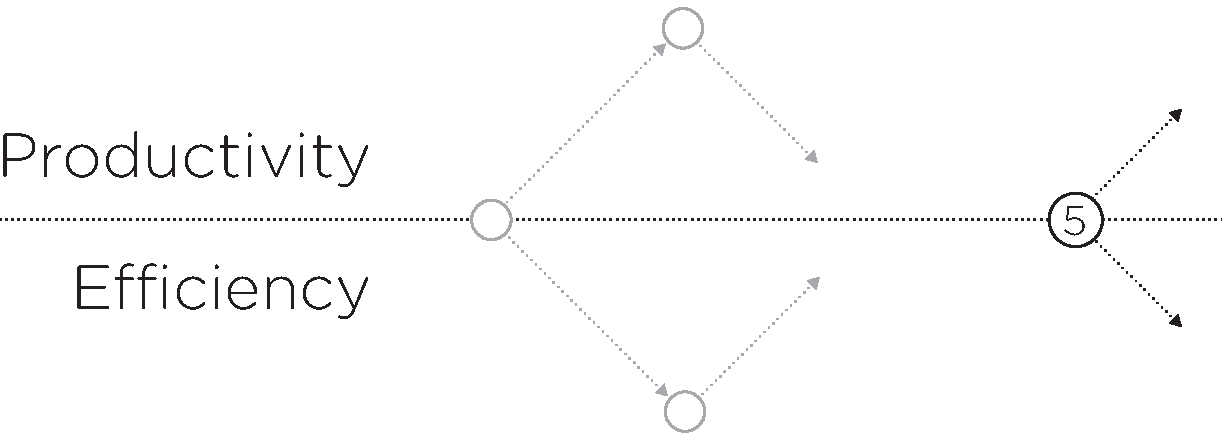
\includegraphics[width=0.6\textwidth]{../resources/state-of-the-art-5.pdf}
% \end{center}
% \end{figure}

\section{Proposition} \label{chapter4:proposition}

This thesis proposes a platform allowing a seamless shift of focus to follow the development of a web application from the productivity required in the early beginning until the efficiency required during maturation.

Developers start a project without compromises on productivity.
The language targets an event-driven execution model.
And they continuously transform their implementation to target the more efficient pipeline architecture.

% The proposed platform allows to develop applications targeting an event-driven platform allowing productivity, and transforms them so as to execute them on a pipeline architecture allowing efficiency.
% It is based on the transformation of an event-driven program to target a pipeline architecture.

% The event-driven platform is embodied by Javascript for the implementation of this thesis.
% \textit{Node.js} is an efficient event-driven execution model to implement a web application.
% Javascript features higher-order programming, dynamic typing and a global memory abstraction.
% Because of these features, it is very productive.
% It makes Javascript a language of choice to develop web applications.

\textit{Node.js} implements Javascript, a productivity language, with an event driven execution model to implement web applications with decent performances.
However, the performance of this execution model is limited by the sequentiality of execution required to preserve exclusivity of memory accesses.
The pipeline execution model overstep this performance limitation.
It enforces memory isolation between stages allowing the parallel execution required for efficiency.
But this isolation limits the productivity because it avoids higher-order programming.
The difference in the memory abstractions between the two execution models is illustrated in figure \ref{fig:difference}.

\begin{figure}[h!]
\begin{center}
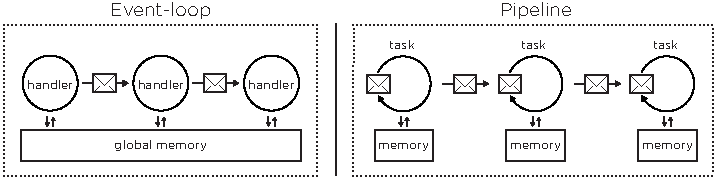
\includegraphics[width=0.9\textwidth]{../resources/models-difference.pdf}
\end{center}
\caption{Differences of memory abstraction}
\label{fig:difference}
\end{figure}


% \subsection{Equivalence}
% The difference of memory model between the two execution model is illustrated in figure \ref{fig:mem-equivalence}.
Despite this difference, these two execution models present an interesting similarity.
They both organize the execution as a sequence of tasks causally scheduled. %, as illustrated in figure \ref{fig:run-equivalence}.
This thesis proposes an equivalence between these two execution models based on this similarity.
Following this equivalence, it proposes a compiler that distributes the global memory into isolated stages of the pipeline.
% with message passing.
% As explained below, the concurrency model of the event-loop execution model, and the parallel approach of the pipeline execution model are very similar.
Concretely, it transforms a mono-threaded, event-driven application to run on a parallel pipeline architecture.

\subsection{Continuous Development}

%It proposes this equivalence as a solution to allow the same platform to propose a continuity of compromises between productivity and efficiency.
This transformation allows a continuity of compromises between productivity and efficiency to seamlessly follow the shift of focus during development.

% Developers keep two organizations of the implementations of an application.
% The organization based on event-driven execution model assures productivity whereas the transformation targeting the pipeline architecture helps improve efficiency.




% Developers keep two organizations of the implementation of an application. %, allowing them to start with productivity, and seamlessly abandon it for efficiency as the project matures.
% The productive organization is based on the event-driven execution model.
% It helps to maintain the application.
% The efficient organization is the transformed application targeting the pipeline execution model.

At first, the focus remains on the productivity of development rather than the efficiency of execution.
The development begins with the event-driven model to take advantage of the productivity of the global memory abstraction.
% and the asynchronous control flow of the event-driven execution model.
The execution resulting from the transformation is as efficient as the original event-driven execution model.

During the maturation of the application, the focus continuously shift towards efficiency.
The transformation distribute the global memory into isolated stages as much as possible.
It allows developer to identify the dependencies in this global memory avoiding the distribution.
They can identify these dependencies, and arrange the implementation accordingly to allow parallelism.
It helps developers to enforce efficiency through continuous iteration, instead of disruptive shifts of technology.

% The next paragraphs introduce this equivalence.


% \begin{figure}[h!]
% \begin{center}
% 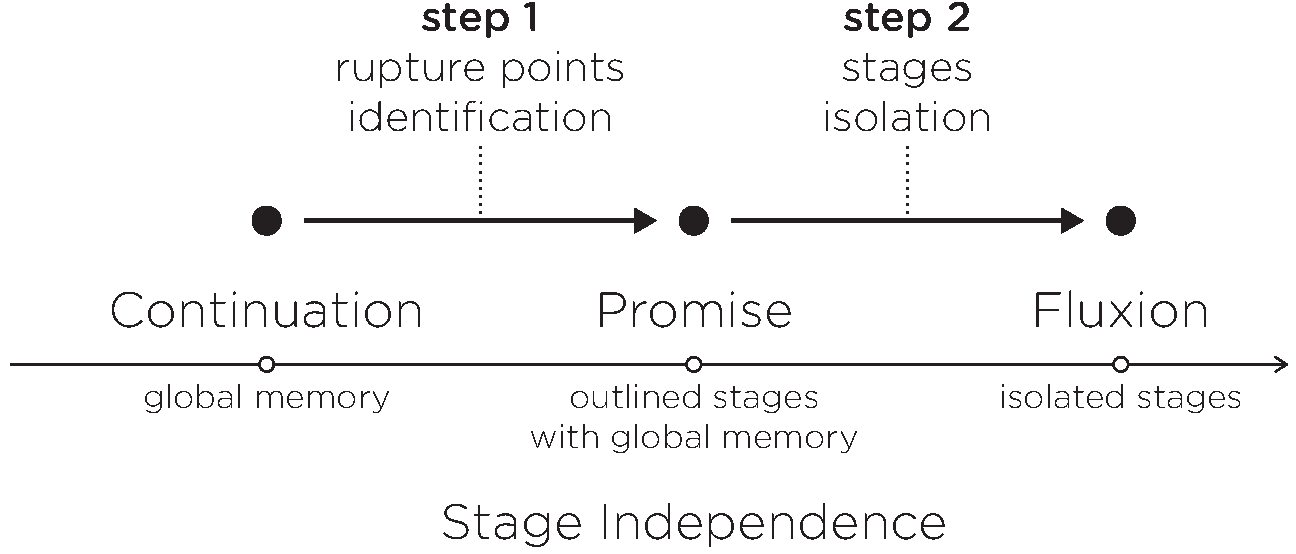
\includegraphics[width=0.7\textwidth]{../resources/roadmap.pdf}
% \end{center}
% \caption{Roadmap}
% \label{fig:roadmap}
% \end{figure}

\subsection{Equivalence} \label{chapter4:equivalence}

% The goal of this thesis is not to propose a new high-level language but to automate the architectural shift.
% The next paragraphs introduces the equivalence
The equivalence between these two execution models is broken down in two steps. %, as illustrated in figure \ref{fig:roadmap}.
The first step identifies the stages in the control flow, by detecting rupture points between them.
% The first step identifies the rupture points in the control flow separating the stages of the pipeline.
The second step enforces isolation of memory between these stages, and replaces synchronization with message passing to preserve the invariance.
% invariance through message passing.

\subsubsection{Execution Independence}

\begin{wrapfigure}{R}{0.4\textwidth}
  \centering
  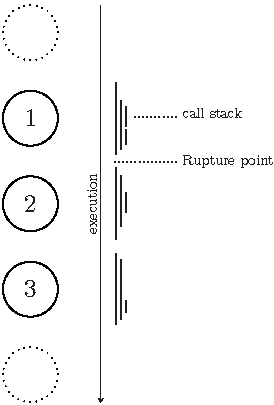
\includegraphics[height=0.5\textwidth]{../resources/rupture-point.pdf}
  \caption{Rupture point}
  \label{fig:rupture-point}
  \vspace{-40pt}
\end{wrapfigure}

% \begin{floatingfigure}[r]{0.33\textwidth}
%   \label{fig:rupture-point}
%   \centering
%   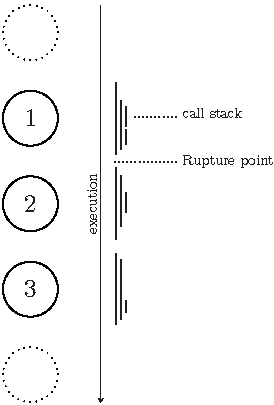
\includegraphics[height=0.4\textwidth]{../resources/rupture-point.pdf}
%   \caption{Rupture point}
% \end{floatingfigure}

% The pipeline architecture enforces the memory isolation between stages.
In the pipeline architecture, each stage has its own thread of execution independent from the others.
Whereas in the event-driven execution model, the handlers are executed sequentially.
% the execution flow jumps from one concurrent handler to the other to execute them sequentialy.
%  because of the continuation passing style and the common memory store.
% The message passing linking the callbacks is transparently handled by the event-loop.
Despite this difference, the execution of a handler is as independent as the execution of a stage of a pipeline.
The call stacks of two handlers are isolated, as illustrated in figure \ref{fig:rupture-point}.
Indeed, a handler holds the execution until its call stack is empty, when all synchronous function calls terminates. Only then it yields the execution to the event-loop, which schedule the next handler.
A rupture point separates the call stacks of two handlers.

For simplification, the figures \ref{fig:rupture-point} illustrates a rupture point with only two interleaving chains of handlers, but there could be many more chains interleaving.
Each chain is comparable to a thread in multi-thread programming.
The two chains in figure \ref{fig:rupture-point} are 
$\to$
\circled{\fontsize{12pt}{10pt}\selectfont\figcapfont 1} $\to$
\circled{\fontsize{10pt}{10pt}\selectfont\figcapfont 2} $\to$ and
\dotcircled{\textcolor{white}{0}} $\to$
\dotcircled{\textcolor{white}{0}} $\to$
\dotcircled{\textcolor{white}{0}}.
And in figures \ref{fig:sequential-scheduling},  \ref{fig:causal-scheduling}, \ref{fig:memory-update} and \ref{fig:sequential-execution}, they are 
$\to$
\circled{\fontsize{12pt}{10pt}\selectfont\figcapfont 1} $\to$
\circled{\fontsize{10pt}{10pt}\selectfont\figcapfont 3} $\to$ and
\dotcircled{\textcolor{white}{0}} $\to$
\circled{\fontsize{10pt}{10pt}\selectfont\figcapfont 2} $\to$
\dotcircled{\textcolor{white}{0}}.

\subsubsection{Rupture points} \label{chapter5:flx-compiler:analyzer:rupture}

A rupture point is a call of a loosely coupled function.
It is an asynchronous call without subsequent synchronization with the caller.
This asynchronous function call is equivalent to a data-flow between two stages in the pipeline architecture.
The parent sends a message to the child handler containing the result of the asynchronous function call it initiated.
The event-driven execution model expects callback to send the message and continue the execution once the asynchronous call completes.

\paragraph{Callbacks, Listeners and Continuations}

A callback is a function passed as a parameter to a function call.
It is not inherently asynchronous.
Only two kinds of callbacks are asynchronous, listeners and continuations.
They are invoked to continue the execution with data not yet available synchronously, in the caller context.
Listeners listen to a stream of events, hence are invoked multiple times.
Whereas continuations are invoked only once to continue the execution after an asynchronous operation completes.
The two corresponding types of rupture points are \textit{start} and \textit{post}.

\textbf{Start rupture points} (listeners) are on the border between the application and the outside, continuously receiving incoming user requests.
An example of a start rupture point is in listing \ref{lst:source}, between the call to \texttt{app.get()}, and its listener \texttt{handler}.
These rupture points indicate the input of a data stream in the program, and the beginning of a chain of fluxions to process this stream.

\textbf{Post rupture points} (continuations) represent a continuity in the execution flow after an asynchronous operation yielding a unique result, such as reading a file, or a database.
An example of a post rupture points is in listing \ref{lst:source}, between the call to \texttt{fs.readFile()}, and its continuation \texttt{reply}.




% The rupture between the call stacks of two handlers is indicated by an asynchronous function call in the parent handler defining a children handler as a continuation or a listener.
% The asynchronous function call - the callee - between the caller and its continuation represents a rupture between the two call stacks.
% And the call stack of the continuation is independent from the call stack of the caller and the callee.

% TODO Definition of the two types of rupture points

% Both the pipeline architecture and the event-loop present these rupture points.
The detection of rupture points allows to retrieve the data-flow and the stages for a pipeline architecture from the implementation following the event-loop model.
% To allow the transformation from one to the other,
% The proposed platform detects rupture points defining stages. %, and distributes the global memory into them.
The implementation of this detection is fully addressed in the next chapter, in sections \ref{chapter5:due:compiler} and \ref{chapter5:flx:compiler}.
% It presents the extraction of a pipeline of concurent tasks from a Javascript application.
% Such pipeline is similar to the one exposed by Promises.
% The chapter proposes a simpler alternative to the latter called Dues.
However, these stages still require a global memory to communicate.
They can't be executed in parallel without breaking the invariance.





\subsubsection{Invariance}

% This transformation is important on two points.
% The conservation of the invariance.
% The equivalence between the coordinations.

\begin{wrapfigure}{L}{0.5\textwidth}
  \begin{minipage}[t]{0.23\textwidth}
    \centering
    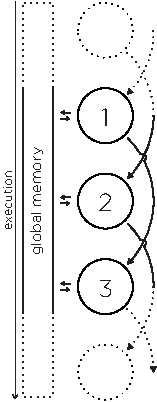
\includegraphics[page=1, height=2\linewidth]{../resources/invariance.pdf}
    \caption{Sequential scheduling}
    \label{fig:sequential-scheduling}
  \end{minipage}
  \hfill
  \vrule
  \hfill
  \begin{minipage}[t]{0.23\textwidth}
    \centering
    \includegraphics[page=2, height=2\linewidth]{../resources/invariance.pdf}
    \caption{Causal scheduling}
    \label{fig:causal-scheduling}
  \end{minipage}
\end{wrapfigure}

A global memory requires the sequential scheduling of handlers to assure exclusivity of access, as illustrated in figure \ref{fig:sequential-scheduling}. % which implies the total scheduling with a queue, as illustrated in figure \ref{fig:total-scheduling}.
The global memory is the only reason for this sequential execution.
% If it could somehow be replace by message-passing, the handlers could be scheduled causally and executed in parallel.
Yet, the causal scheduling of tasks is sufficient to assure the correctness of the execution.

Message passing only requires causal scheduling of handlers which allows parallelism, as illustrated  in figure \ref{fig:causal-scheduling}.
% The sequential execution is imposed by the global memory, not by the causality between handlers.
If the handlers didn't rely on the global memory, they could be executed in parallel, as long as their causalities are respected.
Following some rules, it is possible to replace their global memory usage with message-passing, and parallel their execution.

% \begin{figure}%{L}%{0.5\textwidth}
%   \begin{minipage}[t]{0.23\textwidth}
%     \label{fig:sequential-scheduling}
%     \centering
%     \includegraphics[page=3, height=2\linewidth]{../resources/invariance.pdf}
%     \caption{Message passing memory update}
%   \end{minipage}
%   \hfill
%   \vrule
%   \hfill
%   \begin{minipage}[t]{0.23\textwidth}
%     \label{fig:causal-scheduling}
%     \centering
%     \includegraphics[page=4, height=2\linewidth]{../resources/invariance.pdf}
%     \caption{Sequential execution}
%   \end{minipage}
%   % \vspace{-150pt}
% \end{figure}


\subsubsection{Transformation}

\begin{wrapfigure}{R}{0.5\textwidth}
  \begin{minipage}[t]{0.23\textwidth}
    \centering
    \includegraphics[page=3, height=2\linewidth]{../resources/invariance.pdf}
    \caption{Message passing memory update}
    \label{fig:sequential-scheduling}
  \end{minipage}
  \hfill
  \vrule
  \hfill
  \begin{minipage}[t]{0.23\textwidth}
    \centering
    \includegraphics[page=4, height=2\linewidth]{../resources/invariance.pdf}
    \caption{Sequential execution}
    \label{fig:causal-scheduling}
  \end{minipage}
\end{wrapfigure}

% \begin{wrapfigure}{R}{0.25\textwidth}
%   \centering
%   \includegraphics[page=3, height=2\linewidth]{../resources/invariance.pdf}
%   \caption{Message passing memory update}
%   \label{fig:sequential-scheduling}
%   \vspace{-50pt}
% \end{wrapfigure}

% \begin{wrapfigure}{R}{0.25\textwidth}
%   \centering
%   \includegraphics[page=4, height=2\linewidth]{../resources/invariance.pdf}
%   \caption{Sequential execution}
%   \label{fig:causal-scheduling}
%   \vspace{-50pt}
% \end{wrapfigure}

\paragraph{Rule \#1 Scope}
If an handler uses a variable between the reception of two data, then it needs to store it independently of the global memory.
The reliance on this memory imposes the handler to not be reentrant.
There cannot be several instances of its execution.
The stream of incoming data must be processed sequentially.


\paragraph{Rule \#2 Stream}
If two handlers causally related rely on the same memory region, the causal relation assures the exclusivity of access. Therefore, the global memory can be replaced by sending the updated memory in the data-flow.
As illustrated in figure \ref{fig:memory-update}, the upstream handler \circled{\fontsize{12pt}{10pt}\selectfont\figcapfont 1} communicates the memory update to the downstream handler \circled{\fontsize{10pt}{10pt}\selectfont\figcapfont 3}.
And each handler has access only to its own memory.

\paragraph{Rule \#3 Share}
However, if the downstream handler modifies this memory, it is not possible to isolate it.
The upstream handler cannot be notified in time of this modification.
Indeed, the upstream handler might already be processing the next datum in the stream.
Moreover, if two handlers not causally related rely on the same memory region, they can access it in any order.
They need to be scheduled sequentially to maintain the exclusivity of access, as illustrated in figure \ref{fig:sequential-execution}.

\separator

By distributing the global memory following these rules, the sequential scheduling can be loosen while preserving invariance to parallelize the execution.
This distribution - hence the parallelization - only depends on the memory dependencies between handlers.
Of course, at first, the dependencies will remain tight as the focus is on productivity.
But, developers can continuously iterate on implementation to loosen the dependencies and improve efficiency.

The implementation of the distribution of the global memory is fully addressed in next chapter, in section \ref{chapter5:flx:isolation}.




% As seen in the previous section, a sequential execution of handlers is interleaved by rupture points.




% Therefore, in the correctness of the execution, the ordering allowed by the global memory can be mapped to an equivalent message passing ordering.
% And it is possible to transform the global memory coordination into message passing.
% Given that the tasks are independent and communicate by messages.

% This result was used by Lamport to prove the correctness of distributed systems.
% Yet, to preserve the correctness as expressed by the developer, it is important to preserve the invariance provided by the global memory.
% The global memory needs to be distributed into each of the stages of the pipeline, so that each stage have an exclusive access to its memory.

% Moreover to assure the missing coordinations assured by the shared memory between the stages, the stages need to provide an equivalent coordination with message passing.





% \subsubsection{Transformation}

\paragraph{From Event-loop to Pipeline}

Concretely, this transformation turns handler from the event-driven execution models into stages of the pipeline, as illustrated in figure \ref{fig:run-equivalence}.
And it distributes the global memory  into these different stages, as illustrated in figure \ref{fig:mem-equivalence}.
The details of these two execution models important for this transformation are presented in the next section.

\begin{figure}
  \begin{minipage}[t]{0.45\textwidth}
    \centering
    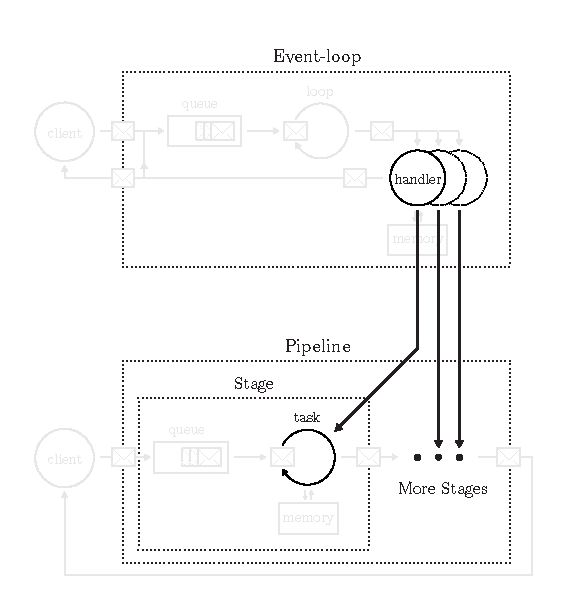
\includegraphics[width=\linewidth]{../resources/run-equivalence.pdf}
    \caption{Equivalence between handlers and tasks}
    \label{fig:run-equivalence}
  \end{minipage}
  \hfill
  \vrule
  \hfill
  \begin{minipage}[t]{0.45\textwidth}
    \centering
    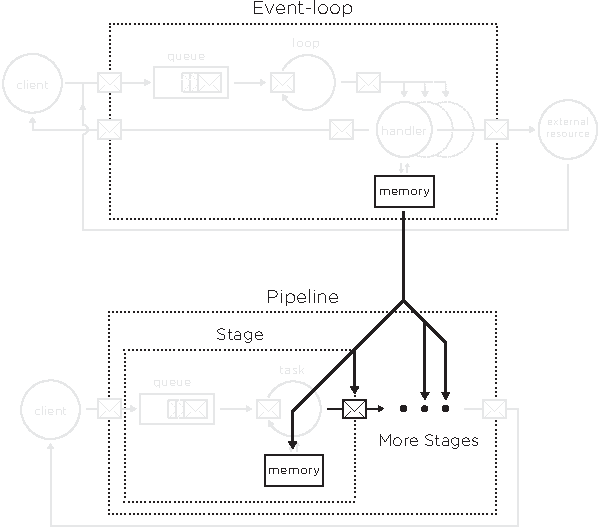
\includegraphics[width=\linewidth]{../resources/mem-equivalence.pdf}
    \caption{Distribution of the global memory abstraction with message passing}
    \label{fig:mem-equivalence}
  \end{minipage}
\end{figure}



% The invariance holds for the whole memory during the execution of each callback.
% As I explained in the previous section, this invariance is required to allow the concurrent execution of the different tasks.
% On the other hand, the invariance is explicit in the pipeline architecture, as all the stages have isolated memories.
% The coordination between these isolated process is made explicit by the developer through message passing.

% I argue that the state coordination between the callbacks requireing a global memory could be replaced by the message passing coordination used manually in the pipeline architecture.
% I argue that not all applications need concurrent access on the state, and therefore, need a shared memory.
% % Specifically, I argue that each state region remains roughly local to a stage during its modification.
% \nt{TODO review that, I don't know how to formulate these paragraphs. Identify the state and the data in the global memory.}

% \subsubsection{Transformation}

% This equivalence should allow the transformation of an event loop into several parallel processes communicating by messages.
% In this thesis, I study the static transformation of a program, but the equivalence should also hold for a dynamic transformation.
% I present the analyzis tools I developed to identify the state and the data from the global memory.

\section{Execution Models} \label{chapter4:execution-models}

The event-driven execution model and the pipeline execution model were already briefly presented in chapter \ref{chapter2}, section \ref{chapter2:web-as-a-platform:web-servers}, page \pageref{chapter2:web-as-a-platform:web-servers}.
The next paragraphs dive into the details of each execution model in regard of the transformation.

\subsection{Event-Driven Execution Model} \label{chapter4:event-driven}

The event-driven execution model processes a queue of asynchronous events by cooperatively scheduling handlers.
To respond to an event, the associated handler can directly respond to the source of the event.
Or it can request an external resource, and chain another handler to later process the initial event with the resource response, as illustred in figure \ref{fig:cont-chain}.
The developer defines each handler as a continuation and defines their causality using the continuation passing style \cite{Wand1980,Haynes1984}.


% \begin{figure}
%   % \centering
%   \textfig{%
%     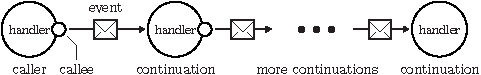
\includegraphics[width=0.8\linewidth]{../resources/cont-chain.pdf}%
%     \caption{Chain of continuations}%
%     \label{fig:cont-chain}%
%   }
% \end{figure}

\subsubsection{Continuation Passing Style} \label{chapter4:event-loop:continuation}

% A callback is a function passed as a parameter to a function call.
% It is invoked by the callee to continue the execution with data not available in the caller context.
% We distinguish three kinds of callbacks.

% \begin{description}
%   \item[Iterators] are functions called for each item in a set, often synchronously.
%   \item[Listeners] are functions called asynchronously for each event in a stream.
%   \item[Continuations] are functions called asynchronously once a result is available.
% \end{description}

% In a synchronous paradigm, the sequentiality of the execution flow is trivial.
% An operation needs to complete before executing the next one.
% In an asynchronous paradigm, parallelism is trivial, but the sequentiality of operations needs to be explicit.

% A continuation is the functional way of defining the causality between two tasks \cite{Wand1980,Haynes1984}.
A continuation is a function passed as an argument to a function call.
% The caller is able to continue the execution while the callee runs in background.
The continuation is invoked after the completion of the callee, to continue the execution. % as soon as possible and process the result; hence the name continuation.
In the event-driven execution model, the continuation is invoked as a new handler, to avoid blocking the caller until its completion.
% It provides a necessary control over the asynchronous execution flow.
% It also brings a control over the data flow which essentially replaces the \texttt{return} statement at the end of a synchronous function.
At its invocation, the continuation retrieves both the caller context and the result of the callee through a closure.
Listing \ref{lst:continuation} illustrates an example of continuation in \textit{Node.js}.

% The convention on how to hand back the result must be common for both the callee and the continuation.
% For example, in \textit{Node.js}, the signature of a continuation uses the \textit{error-first} convention.
% % \ftnt{https://docs.nodejitsu.com/articles/errors/what-are-the-error-conventions}
% % \ftnt{http://programmers.stackexchange.com/questions/144089/different-callbacks-for-error-or-error-as-first-argument} convention.
% The first argument contains an error or \texttt{null} if no error occurred; then follows the result.
% Listing \ref{lst:continuation} is a pattern of such a continuation.
% However, continuations don't impose any conventions; indeed, other conventions are used in the browser.

\begin{code}[js, %
             caption={Example of a continuation}, %
             label={lst:continuation}] %
callee(input, function continuation(error, result) {
  if (error)
    throw error;
  // ... modify result
  console.log(result);
});
\end{code}

% % The continuation allows to continue the execution sequentially, after the result of \textit{my_fn} is available.
% % When continuations are defined inside the call, like \textit{continuation}, the sequence of deferred execution results in an intricate imbrication of calls and continuations, like in listing \ref{lst:cbhell}.
% The callback hell occurs when many asynchronous calls are arranged to be executed sequentially.
% Each consecutive operation adds an indentation level, because it is nested inside the continuation of the previous operation.
% % That is when each caller must wait for the result before calling the next function.
% It produces an imbrication of calls and function definitions, as shown in listing \ref{lst:cbhell}.

Asynchronous continuations cannot be composed to chain their execution like synchronous functions, as illustrated in listing \ref{lst:cbhell}.
This nested construction is sometime difficult to follow.
% The continuation passing style lacks the chained composition of multiple asynchronous operations.
% It forces to stack calls of continuations, as illustrated in listing \ref{lst:cbhell}.
Promises improve continuations to allow this composition.
They allow to arrange a sequence of asynchronous operations in a chain, similar to a pipeline.

\begin{code}[js, %
             caption={Example of a sequence of continuations}, %
             label={lst:cbhell}] %

callee(input, function continuation(error, result) {
  if (error)
    throw error;
  // ... modify result
  nestedCallee(result, function continuation(error, nestedResult) {
    if (error)
      throw error;
    // ... modify result
    superNestedCallee(nestedResult, function continuation(error, superNestedResult) {
      // ... and so on ...
    }
  });
});
\end{code}

\subsubsection{Promise} \label{chapter4:event-loop:promise}

% TODO insert these :
% Promise also provide few methods to enhance the asynchronous control flow tools\footnote{\texttt{all} and \texttt{race}}.
% There is, in Javascript, numerous Promise implementations\footnote{37 different implementations in Javascript \url{https://github.com/promises-aplus/promises-spec/blob/master/implementations.md}}.

% This section is based on the Promises section of the specification in ECMAScript 6 Harmony\ftnt{https://people.mozilla.org/~jorendorff/es6-draft.html\#sec-promise-objects} and the Promises page on the Mozilla Developer Network\ftnt{https://developer.mozilla.org/en/docs/Web/JavaScript/Reference/Global_Objects/Promise}.

% In a synchronous paradigm, the sequentiality of the execution flow is trivial.
% In the asynchronous paradigm, the control over the asynchronous execution flow is defined with continuations.
% In the asynchronous paradigm, this control is provided by continuations.
% Promises provide a unified control over the execution flow for both paradigms.
% The ECMAScript 6 specification\ftnt{https://people.mozilla.org/~jorendorff/es6-draft.html\#sec-promise-objects} defines
A Promise is used as a placeholder for the eventual outcome of a deferred (and possibly asynchronous) operation.
Listing~\ref{lst:then} illustrates a simple promise.
% A Promise is an object returned by a function to represent its result
In Javascript, promises expose a \texttt{then} method which expects a continuation to continue the execution with the result of the deferred operation. %; this result being synchronously or asynchronously available.
This method allows to chain Promises one after the other, as illustrated in listing~\ref{lst:promises-sequence}.

% However, unlike continuations, the Promises specification imposes a convention on how to handle the result.
% Because it is possibly unavailable synchronously, it still requires a continuation to defer the execution when the result is made available.
% A promise requires two continuations to defer the execution in case of errors.
% These two continuations are passed to the \texttt{then} method of the promise, like illustrated in listing \ref{lst:then}.

% As a result of this difference, Promises and continuations use two different conventions to handle errors and results.
% The two conventions are illustrated in listings \ref{lst:continuation} and \ref{lst:then}.

\begin{code}[js, %
             caption={Example of a Promise}, %
             label={lst:then}] %
var promise = callee(input)

promise.then(function onSuccess(result) {
  console.log(result);
}, function onError(error) {
  throw error;
});
\end{code}

% Continuations lack the chained composition of asynchronous operations.
% Promises are designed to fill the lack of chained composition from continuations.
% They allow to arrange successions of asynchronous operations as a chain of continuations, by opposition to the imbrication of continuations illustrated in listing \ref{lst:cbhell}.
% That is to arrange them, one operation after the other, in the same indentation level.
% The \texttt{then} method synchronously returns a Promise linked with the Promise asynchronously returned by its continuation.
% This link allow to compose chains of asynchronous operations.


% The functions \texttt{callee\_promise\_2} and \texttt{callee\_promise\_3} return promises when they are executed.
% They are executed asynchronously, so these promises are not available synchronously.
% The method \texttt{then} synchronously returns intermediary Promises to bridge with the asynchronous promises.
% The former resolves when the latter resolves.
% The latter resolve only when the former resolve.
% This behavior allows to arrange the continuations as a flat chain of calls, instead of an imbrication of continuations.

\begin{code}[js, %
             caption={Example of a chain of Promises}, %
             label={lst:promises-sequence}] %
callee_promise_1(input)
.then(callee_promise_2, onError)
.then(callee_promise_3, onError)
.then(console.log, onError);

function onError(error) {
  throw error;
}
\end{code}

% The Promises syntax is more concise, and also more readable because it is closer to the familiar synchronous paradigm.
% Indeed, Promises allow to arrange both the synchronous and asynchronous execution flow with the same syntax.
Promises allow to easily arrange the execution flow in parallel or in sequence according to the required causality.
% This control over the execution leads to a modification of the control over the data flow.
Programmers are encouraged to arrange the computation as series of steps to process incoming events and yield outcoming events.
In this sense, Promises are an intermediate step toward the pipeline execution model.



\subsection{Fluxional Execution Model} \label{chapter4:flx-model}

The fluxional execution model is inspired by the pipeline architecture.
It is the target for the transformation presented in this thesis.
It executes programs written in the fluxional language, whose grammar is presented in figure \ref{fig:flx-lang}.
It intends to provide scalability to web applications with a granularity of parallelism at the function level.

The functions of an application $\bnfpn{program}$ are encapsulated in autonomous execution containers named \textit{fluxions} $\bnfpn{flx}$.

\begin{figure}[h]
\vspace{-0.6\baselineskip}
\begin{bnf*}
  \bnfprod{program}    {\bnfpn{flx} \bnfor \bnfpn{flx} \bnfsp \bnftd{eol} \bnfsp \bnfpn{program}}\\
  \bnfprod{flx}        {\bnfts{\texttt{flx}} \bnfsp \bnfpn{id} \bnfsp \bnfpn{tags} \bnfsp \bnfpn{ctx} \bnfsp \bnftd{eol} \bnfsp \bnfpn{streams} \bnfsp \bnftd{eol} \bnfsp \bnfpn{fn}}\\
  \bnfprod{tags}       {\bnfts{\texttt{\&}} \bnfsp \bnfpn{list} \bnfor \bnftd{empty string}}\\
  \bnfprod{streams}    {\bnfts{\texttt{null}} \bnfor \bnfpn{stream} \bnfor \bnfpn{stream} \bnfsp \bnftd{eol} \bnfsp \bnfpn{streams}}\\
  \bnfprod{stream}     {\bnfpn{type} \bnfsp \bnfpn{dest} \bnfsp [\bnfpn{msg}]}\\
  \bnfprod{dest}       {\bnfpn{list}}\\
  \bnfprod{ctx}        {\bnfts{\texttt{\{}} \bnfpn{list} \bnfts{\texttt{\}}}}\\
  \bnfprod{msg}        {\bnfts{\texttt{[}} \bnfpn{list} \bnfts{\texttt{]}}}\\
  \bnfprod{list}       {\bnfpn{id} \bnfor \bnfpn{id} \bnfsp \bnfts{,} \bnfsp \bnfpn{list}}\\
  \bnfprod{type}       {\bnfts{\texttt{>}\texttt{>}} \bnfor \bnfts{\texttt{-}\texttt{>}}}\\
  \bnfprod{id}         {\bnftd{Identifier}}\\
  \bnfprod{fn}         {\bnftd{Source language with~} \bnfpn{stream} \bnftd{~placeholders}}\\
\end{bnf*}
\vspace{-2.5\baselineskip}
\caption{Syntax of a high-level language to represent a program in the fluxional form}
\label{fig:flx-lang}
\end{figure}


% The following paragraphs present the \textit{fluxions} and the messaging system to carry the communications between \textit{fluxions}.
% , and then an example application using this execution model.

% \subsubsection{Fluxions and Messaging System}

\subsubsection{Fluxion}

A \textit{fluxion} $\bnfpn{flx}$ is named by a unique identifier $\bnfpn{id}$ to receive messages, and might be part of one or more groups indicated by tags $\bnfpn{tags}$.
A \textit{fluxion} is composed of a processing function $\bnfpn{fn}$, and a local memory called a \textit{context} $\bnfpn{ctx}$.

At a message reception, the \textit{fluxion} modifies its \textit{context}, and sends messages to downstream \textit{fluxions} on its output streams $\bnfpn{streams}$.
The \textit{context} stores the state on which a \textit{fluxion} relies between two message receptions, similarly to the actors model.
The messaging system queues the output messages for the event loop to process them later by calling the downstream \textit{fluxions}.

% And the communications are similar to the dataflow programming model, which allows to reason on the throughput of these streams, and to react to load increases \cite{Bartenstein2014}.

In addition to message passing, the execution model allows \textit{fluxions} to communicate by sharing state between their \textit{contexts}.
The fluxions that need this synchronization are grouped with the same tag, and loose their independence.

\subsubsection{Streams}

There are two types of streams, \textit{start} and \textit{post}, which correspond to the nature of the rupture point producing the stream.
A \textit{start} rupture point starts a chain of continuations, while a \textit{post} rupture point is a continuation in a chain.
\textit{Start} streams are indicated with a double arrow ($\to$ \hspace{-1.4em} $\to$ or \texttt{>>}) and \textit{post} streams with a simple arrow ($\to$ or \texttt{->}).

The variables defined before the \textit{start} are available for the whole chain, and require synchronization for concurrent execution of the same chain.
Whereas the variables defined inside the chain are available only in this chain, and don't require synchronization.
% A variable created within a chain of \textit{post} streams requires more synchronization than a variable created upstream a \textit{start} stream.
The two types and implications of rupture points are further detailed in section \ref{chapter5:flx:compiler}.

\subsection{Examples} \label{chapter4:execution-models:examples}

\subsubsection{Illustration Of The Fluxional Exection Model}

\marginfig{9}{0.4\textwidth}{
  
\includegraphics[height=0.2\textwidth]{../resources/grumpy.png}
}

Even if the fluxional execution model is not designed to directly develop applications, a first application was develop directly with it, to test it.
This application doesn't use the transformation, nor the continuous development advocated in this thesis.
Nonetheless, it is related here to illustrate the basic functioning of the fluxional execution model.

The application is accessible online at \url{http://grumpy.etnbrd.com}, and the source code is available at \url{https://github.com/etnbrd/grumpy}.
And the network of fluxions structuring the applications can be monitored in realtime at \url{http://grumpy.etnbrd.com/console}, as illustrated in figure \ref{fig:grumpy-screenshot}.
The application allows to post anonymous grumbles into chat rooms.
Additionally, a room can subscribe to the grumbles from another room.
The reader is invited to play with this application and the monitoring console to maybe quickly grasp an understanding of the fluxional execution model \footnote{The reader might want to keep in mind that crude languages might be present on the platform. It is available freely on the internet for anyone to express itself.}.

\begin{figure}
  \bigfig{
    \centering
    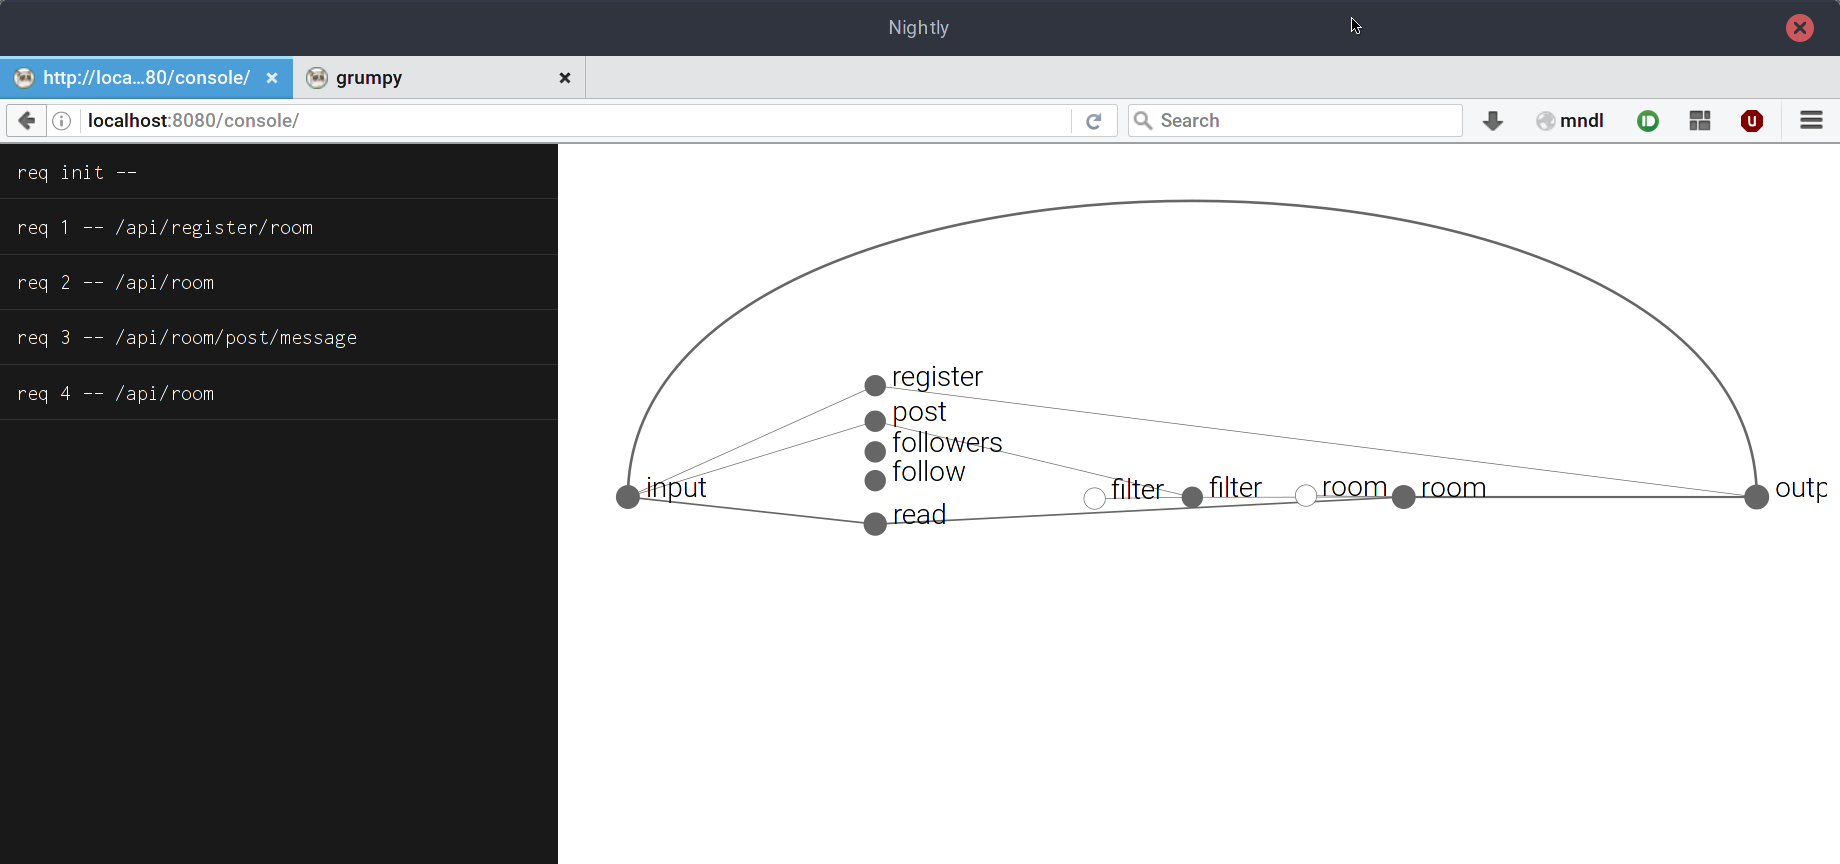
\includegraphics[width=\textwidth]{../resources/grumpy-console.png}
    \caption{Screenshot from the grumpy console}
    \label{fig:grumpy-screenshot}
  }
\end{figure}

The network of fluxions is organized into five layers of stages, traversed by the stream of request from left to right.
The first and last layers are the input and output, connecting the application with the clients.
The second layer contains the fluxions receiving and formatting the request, before passing them to the next layer.
The fluxion in the third layer is a simple filter before posting grumbles.
It is an example of a fluxion modifying a message from the stream.
Finally, each room is instantiated as a new fluxion in the fourth layer, storing the received grumbles in its context.

The left panel logs the requests received by the application, and the path of each request can be traced from stage to stage.

The socket descriptor is stuck with the network interface, hence, it cannot be serialized to flow from one fluxion to another.
Instead, the first and last fluxions share their memory, and each request flows with an id to associate it with its socket descriptor.

This example application was developed before the implementation of the isolation of fluxions in the fluxional execution model.
So it was possible to share their memory by simply sending a memory reference between two fluxions, without grouping them.
This explains the direct link between the input and output fluxions.

The example illustrated in the next paragraphs explains in more details the transformation, and the grouping required for fluxion sharing memory.
And it explains the impact of the memory dependencies on parallelism and scalability.

\subsubsection{Illustration Of The Application Transformation}

The transformation from continuation passing style to the fluxion execution model is now illustrated with a simple web application.

\begin{code}[js,
  caption={Example web application},
  label={lst:source}]
var app = require('express')(),
    fs = require('fs'),
    count = 0; //@\label{lst:source-counter}@

app.get('/', function handler(req, res){ //@\label{lst:source-handler}@
  fs.readFile(__filename, function reply(err, data) {
    count += 1;
    res.send(err || template(count, data)); //@\label{lst:source-send}@
  });
}); //@\label{lst:source-handler-end}@

app.listen(8080);
\end{code}

% \begin{wrapfigure}{r}{0.60\textwidth}
%   \vspace{-25pt}
%   \begin{center}
%     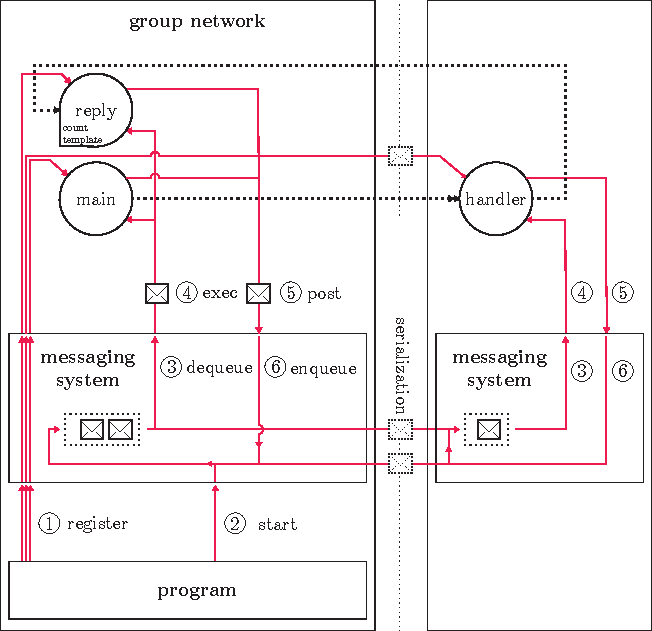
\includegraphics[width=\linewidth]{../resources/schema-message.pdf}
%     \caption{The fluxional execution model in details}
%     \label{fig:MesSys}
%   \end{center}
%   \vspace{-10pt}
% \end{wrapfigure}

% The fluxional execution model is illustrated with an example application presented in listing \ref{lst:source}.
The example application in listing \ref{lst:source} reads a file, and sends it back along with a request counter.
The \texttt{handler} function, line \ref{lst:source-handler} to \ref{lst:source-handler-end}, receives the input stream of requests.
The \texttt{count} variable at line \ref{lst:source-counter} counts the requests, and needs to be saved between two messages receptions.
The \texttt{template} function formats the output stream to be sent back to the client.
The \texttt{app.get} and \texttt{res.send} functions, lines \ref{lst:source-handler} and \ref{lst:source-send}, interface the application with the clients.
Between these two interface functions, there is a chain of three functions to process the client requests : \texttt{app.get} $\to$ \hspace{-1.4em} $\to$ \texttt{handler} $\to$ \texttt{reply}.
This chain of functions is transformed into a pipeline, expressed in the high-level fluxional language in listing \ref{lst:fluxional}.
The transformation process between the source and the fluxional code is explained in chapter \ref{chapter5}, in section \ref{chapter5:flx:compiler}.

\begin{code}[flx, caption={Example application expressed in the high-level fluxional language}, label={lst:fluxional}]
flx main & grp_res
>> handler [res]
  var app = require('express')(),
      fs = require('fs'),
      count = 0;

  app.get('/', >> handler); //@\label{lst:fluxional-streamtohandler}@
  app.listen(8080);

flx handler
-> reply [res]
  function handler(req, res) {
    fs.readFile(__filename, -> reply); //@\label{lst:fluxional-readfile}@
  }

flx reply & grp_res {count, template}
-> null
  function reply(error, data) {
    count += 1; //@\label{lst:fluxional-counter}@
    res.send(err || template(count, data)); //@\label{lst:fluxional-ressend}@
  }
\end{code}

The execution is illustrated in figure \ref{fig:MesSys}.
The dashed arrows between fluxions represent the message streams as seen in the fluxional application.
The plain arrows represent the operations of the messaging system during the execution.
These steps are indicated by numeroted circles.
The \textit{program} registers its fluxions in the messageing system, \circled{1}.
The fluxion \textit{reply} has a context containing the variable \texttt{count} and \texttt{tem\-plate}.
When the application receives a request, the first fluxion in the stream, \textit{main}, queues a \texttt{start} message containing the request, \circled{2}.
This first message is to be received by the next fluxion \textit{handler}, \circled{3}, and triggers its execution, \circled{4}.
The fluxion \textit{handler} sends back a message, \circled{5}, to be enqueued, \circled{6}.
The system loops through steps \circled{3} to \circled{6} until the queue is empty.
This cycle starts again for each new incoming request causing another \texttt{start} message.

\begin{figure}[h!]%
  \textfig{%
    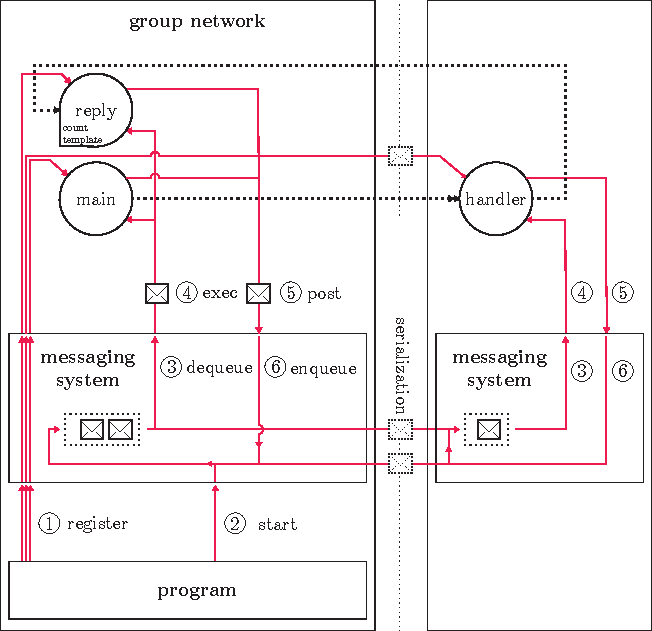
\includegraphics[width=0.7\linewidth]{../resources/schema-message.pdf}%
    \caption{The fluxional execution model in details}%
    \label{fig:MesSys}%
  }%
\end{figure}

The chain of functions from listing \ref{lst:source} is expressed in the fluxional language in listing \ref{lst:fluxional}.
The fluxion \texttt{handler} doesn't have any dependencies, so it can be executed in a parallel event-loop.
The fluxions \texttt{main} and \texttt{reply} belong to the group \texttt{grp\_res}, indicating their dependency over the variable \texttt{res}.
The group name is chosen arbitrarily.
All the fluxions inside a group are executed sequentially on the same event-loop, to protect the shared variables against concurrent accesses.

The variable \texttt{res} is created and consumed within a chain of \textit{post} stream.
Therefore, it is exclusive to one request and cannot be propagated to another request.
It doesn't prevent the whole group from being replicated.
However, the fluxion \texttt{reply} depends on the variable \texttt{count} created upstream the \textit{start} stream, which prevents this replication.
If it did not rely on this variable, the group \texttt{grp\_res} would be stateless, and could be replicated to cope with the incoming traffic.

\separator

This execution model allows to parallelize the execution of an application as a pipeline, as with the fluxion \texttt{handler}.
And some parts are replicated, as could be the group \texttt{grp\_res}.
This parallelization improves the efficiency of the application.
Indeed, as a fluxion contains its state and expresses its dependencies, it can be migrated.
It allows to adapt the number of fluxions per core to adjust the resource usage in function of the desired throughput.

Yet, the parallelization is limited by the dependencies between fluxions.
A developer can ignore these dependencies at first, to focus on productivity.
And then continuously tune the implementation to remove these dependencies and improve efficiency.
This continuous tuning avoids the disruptive shifts of technology required by current platforms.


\section{Conclusion}

This chapter presented the proposition of this thesis : an equivalence between the event-driven execution model and the pipeline execution model for web applications.
The equivalence intends to allows developers to control simultaneously productivity, and efficiency of their implementation.
Because it allows them to continuously have two representations, developers can then choose their compromize, depending on what they are after.
This compromize evolves with the implementation.

The equivalence is based on the event-driven and fluxional execution models presented respectively in section \ref{chapter4:event-driven} and \ref{chapter4:flx-model}.
It relies on the similar pipeline organization shared by these two models.
It detects the rupture points between the stages to extract the pipeline organization from an event-driven implementation.
Then, it isolates these stages so as to allow parallel execution.

We published this work at three occasions.
The core idea of these contribution was briefly presented as a poster in December 2014 at Middleware \cite{Brodu2014}, and then more thouroughly presented in April 2015 at Symposium for Application Computing in the track Practical Aspect of Parallel Programming \cite{Brodu2015a}.
In the meantime, an intermediate step was presented in April 2015, at the AWeS Workshop at the Eurosys Conference \cite{Brodu2015}.
The implementations presented in these papers are reminded in the next section.
